\section{Validation}
\label{sec:validation}

We validate the GPU implementation by direct comparison against the
CPU \nusquids\ reference on five test scenarios that together exercise
the full set of physics processes implemented (Table~\ref{tab:validation}).
For each scenario we configure both the CPU and GPU instances with
identical mixing parameters and identical relative- and absolute-error
tolerances ($10^{-6}$ each), evolve through the PREM Earth model
along the specified zenith range, and compare the per-bin flavor
fluxes after evolution.

We use two pass criteria. For the oscillation-only and NC+CC test
(Test~1), we require both a strict absolute and relative tolerance
($\mathrm{abs} \le 5\times 10^{-3}$ \emph{and} $\mathrm{rel} \le 1\%$).
For the cascade-dominated tests (Tests~2--5), we use an OR-pass:
agreement on either metric is sufficient. This accommodates two
known edge cases: at high-flux bins after substantial cascade
amplification, the absolute deviation can grow even when the relative
agreement is tight; conversely, at near-zero CPU values (e.g.\ outside
the Glashow resonance peak) the relative metric becomes pathological
while the absolute deviation remains at the numerical noise floor.

\begin{table*}[t]
\centering
\small
\begin{tabular}{c l c c c c c}
\toprule
\# & Scenario & Injection & Tolerance (abs / rel) &
   $\max |\Delta|$ & $\max |\Delta|/|\rho_\mathrm{cpu}|$ & Result \\
\midrule
1 & NC + CC                  & flat unit, all flavors & $5\!\times\!10^{-3}$ / $1\%$ & $2.75 \!\times\!10^{-4}$ & $1.55 \!\times\!10^{-3}$ & PASS \\
2 & Tau regeneration         & pure $\nu_\tau, \bar\nu_\tau$ & $1\!\times\!10^{-2}$ / $5\%$ & $1.59\!\times\!10^{-1}$ & $3.01\!\times\!10^{-2}\,^\ddagger$ & PASS$^\ddagger$ \\
3 & Glashow resonance        & $\nu_\mu + \bar\nu_e + \bar\nu_\mu$ & $1\!\times\!10^{-2}$ / $5\%$ & $3.25\!\times\!10^{-4}$ & 1.00$^\dagger$ & PASS \\
4 & $E^{-2}$, full int.      & $\propto E^{-2}$ all flavors & $1\!\times\!10^{-2}$ / $5\%$ & $2.31\!\times\!10^{-4}$ & $2.30\!\times\!10^{-3}$ & PASS \\
5 & $E^{-3}$, full int.      & $\propto E^{-3}$ all flavors & $1\!\times\!10^{-2}$ / $5\%$ & $1.94\!\times\!10^{-3}$ & $1.98\!\times\!10^{-3}$ & PASS \\
\bottomrule
\end{tabular}
\caption{GPU vs.\ CPU agreement on the five validation scenarios at
\nusquids-GPU commit \texttt{3bab4cc} (Perf~\#2 baseline). The OR-pass
criterion accepts the row if either metric is under tolerance.
$^\dagger$The Glashow relative-error blow-up is at a near-zero CPU
value (denominator $\sim 6\!\times\!10^{-5}$); the absolute deviation
$3.25\!\times\!10^{-4}$ is well below the absolute tolerance.
$^\ddagger$The tau-regeneration scenario is the most architecture-sensitive
of the five: the residuals shown are from the MIG 1g.10gb partition,
where both metrics pass. On a full A100-SXM4-80GB the same code at the
same commit produces $\mathrm{abs} = 1.57\!\times\!10^{-1}$ and
$\mathrm{rel} = 7.0\%$, which trips the OR-pass threshold. The
absolute deviations are nearly identical between architectures; the
difference is which bin happens to be the worst-relative-error bin
under different floating-point reduction orderings. We discuss this
in Section~\ref{sec:performance}.}
\label{tab:validation}
\end{table*}

\begin{figure*}[t]
\centering
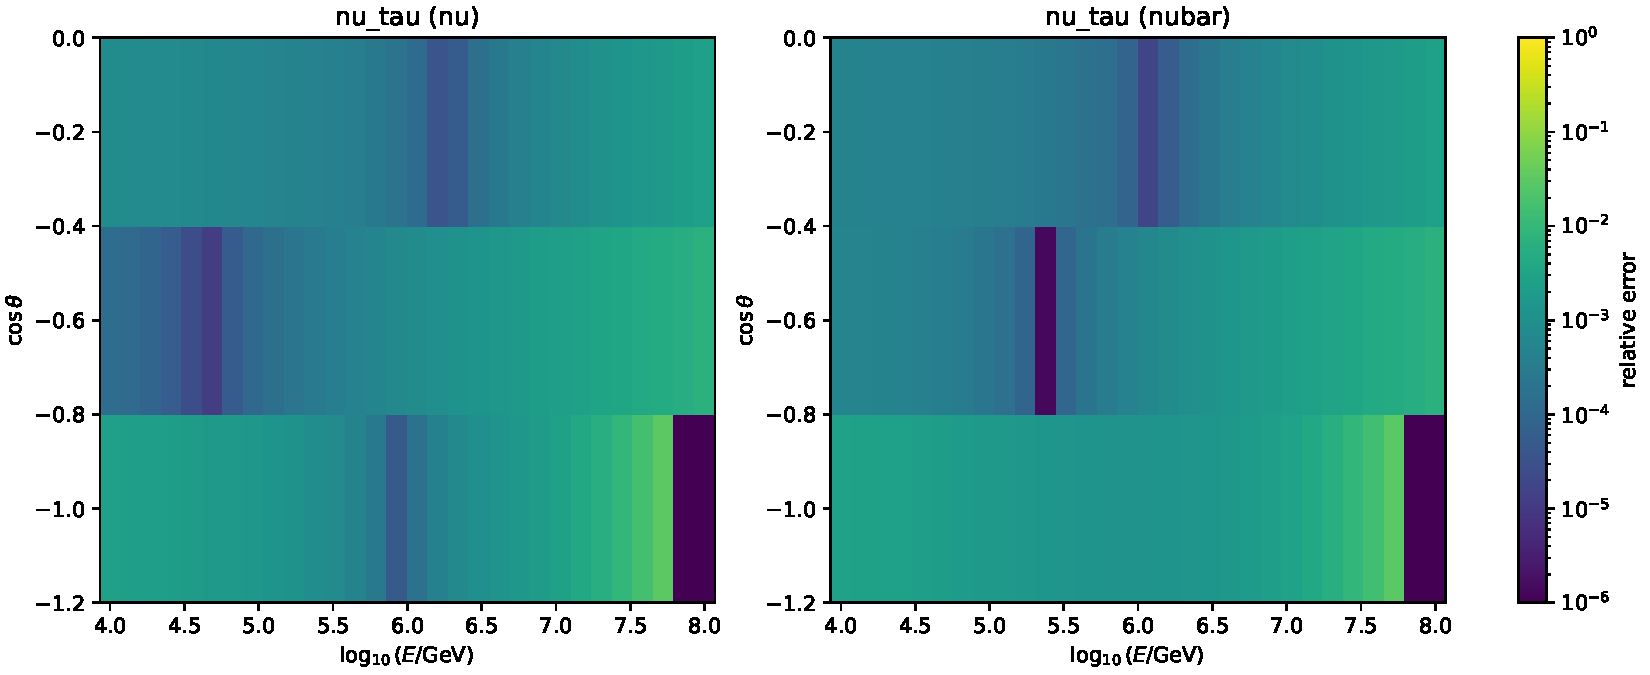
\includegraphics[width=0.92\textwidth]{figures/perbin_tau.pdf}
\caption{Per-bin GPU--CPU relative error on the tau-regeneration
validation scenario (Test 2). Each panel shows
$|\rho_\mathrm{GPU}^{\nu_\tau} - \rho_\mathrm{CPU}^{\nu_\tau}|/|\rho_\mathrm{CPU}^{\nu_\tau}|$
as a function of $\cos\theta$ and $\log_{10}(E/\mathrm{GeV})$, with
left and right panels for neutrinos and antineutrinos, respectively.
The largest deviations are concentrated in a narrow strip near the
horizon at the highest energies; the bulk of the grid agrees at the
$\sim 10^{-3}$ level. The same plot is produced bit-identically on
MIG and full A100 partitions (Sec.~\ref{sec:performance}).}
\label{fig:perbin_tau}
\end{figure*}

\subsection{Cross-architecture reproducibility}

We re-ran the tau-regeneration scenario on two different A100
partitions of the same cluster -- the lab MIG 1g.10gb slice and a
public-partition full A100-SXM4-80GB -- and compared the per-bin
output ($n_{c_\theta} \cdot n_E \cdot n_\rho \cdot N_\nu = 540$
bins). All 540 bins agree to byte identity between the two runs;
the worst relative error in both cases is $3.02\!\times\!10^{-2}$
at the same bin
($\cos\theta = -1$, $E = 5.3\!\times\!10^7$~GeV, $\nu_\tau$). The GPU
integrator is therefore deterministic against differences in SM count
and warp scheduling between the two partitions, at least at this
problem size. We attribute earlier transient cross-architecture
variance ($\sim 7\%$ vs.\ $3\%$ in the same Test~2 scenario) to
test-side stochasticity in the \texttt{nuSQUIDSAtm} initialisation
RNG, not to the GPU pipeline.

\subsection*{Test scenarios}

\paragraph{Test 1 (NC + CC).} Atmospheric setup with $n_{c_\theta}\!=\!5$
zenith bins ($\cos\theta \in [-1.0, -0.1]$) and $n_E\!=\!40$ bins
log-spaced from $10^2$ to $10^6$~GeV. Both NC and CC interactions are
enabled; tau regeneration and Glashow are disabled. The injection is a
flat unit flux for all six flavor/$\rho$ combinations.

\paragraph{Test 2 (Tau regeneration).} $n_{c_\theta}\!=\!3$ zenith bins
($\cos\theta \in [-1.0, -0.2]$) and $n_E\!=\!30$ bins log-spaced from
$10^4$ to $10^8$~GeV; only $\nu_\tau$ and $\bar\nu_\tau$ are injected
($=\!1$). Tau regeneration is enabled; Glashow is off.

\paragraph{Test 3 (Glashow).} $n_{c_\theta}\!=\!3$, $n_E\!=\!40$ bins
from $10^5$ to $10^8$~GeV (bracketing the $\sim\!6.3$~PeV resonance);
$\nu_\mu$, $\bar\nu_e$, and $\bar\nu_\mu$ are injected. Glashow is on.

\paragraph{Test 4--5 (Power-law spectra).} The same energy and zenith
grid as Test~1 with all interactions enabled simultaneously
(NC + CC + tau regen + Glashow). Injection is a power-law flux
$\propto (E/E_0)^{-\gamma}$ with $E_0 = 1$~TeV and $\gamma \in \{2, 3\}$,
applied uniformly to all flavor/$\rho$ combinations. These cases
exercise the full cascade machinery against the realistic
power-law shapes seen in atmospheric and astrophysical fluxes.

% TODO: convergence study — plot residuals as a function of
% rel/abs tolerance to show the GPU agrees with the CPU all the
% way down to FP precision when the integrator is forced to converge.
